\documentclass[11pt,a4paper]{article}
\usepackage[T1]{fontenc}
\usepackage{mathptmx}
\usepackage{courier}
\usepackage[a4paper,margin=2.2cm]{geometry}
\usepackage{float,needspace,graphicx,booktabs,amsmath,xcolor,titlesec,caption,enumitem,microtype}
\usepackage[hidelinks]{hyperref}
\definecolor{navy}{HTML}{14305C}
\definecolor{gold}{HTML}{C8981E}
\titleformat{\section}{\large\bfseries\color{navy}}{\thesection.}{0.5em}{}[{\color{gold}\titlerule[0.6pt]}]
\titlespacing*{\section}{0pt}{10pt}{5pt}
\captionsetup{font=small,labelfont={bf,color=navy}}
\setlength{\parindent}{0pt}\setlength{\parskip}{4pt}
\renewcommand{\baselinestretch}{1.02}
\raggedbottom
\setlength{\textfloatsep}{8pt}\setlength{\intextsep}{7pt}
\graphicspath{{../results/figures/}}
\newcommand{\VFiles}{908}
\newcommand{\VSent}{128}
\newcommand{\VSpk}{104}
\newcommand{\VGroups}{177}
\newcommand{\VLab}{737}
\newcommand{\VMin}{191}
\newcommand{\VPeak}{0.91}
\newcommand{\VShare}{80}
\newcommand{\VAlphaE}{0.17}
\newcommand{\VExample}{3645--186230--0018}
\newcommand{\VRoom}{rm1}
\newcommand{\VMic}{clo}


\begin{document}
\begin{center}
{\color{navy}\rule{\textwidth}{1.2pt}}\\[6pt]
{\LARGE\bfseries\color{navy} Background Classification and Voice Activity Detection on VOiCES}\\[4pt]
{\large Mini Task 9 Report, Digital Speech Processing}\\[6pt]
Natiq Hassan Al Abboody \quad|\quad Student ID: 404131065\\
Instructor: Dr. Mohammad Khalooei \quad|\quad November 2026\\[2pt]
{\color{gold}\rule{\textwidth}{0.8pt}}
\end{center}

\section{Task and data}
This mini task covers three questions on audio recorded in difficult rooms: which background sound is playing, whether a short window contains speech, and, frame by frame, where the speech is (voice activity detection, VAD). The instructor pointed us to the VOiCES corpus~\cite{voices}, in which LibriSpeech sentences are played from a loudspeaker in real rooms and picked up by distant microphones, while a second loudspeaker plays babble, music or television, or nothing.

The full corpus is far too large for this work, so I used the 90-degree subset that Lab41 publishes on GitHub~\cite{subset}. It has \VFiles{} files (about 3.9 hours) of \VSent{} sentences from \VSpk{} speakers, recorded in two rooms with microphones at four positions (close, middle, far and behind). The four background conditions are almost balanced (227 none, 228 babble, 231 music, 222 television). All labels come from the file names, which follow the pattern in the README~\cite{readme}, for example \texttt{...-rm1-musi-sp0242-\allowbreak ch122625-\allowbreak sg0004-\allowbreak mc05-\allowbreak stu-\allowbreak far-\allowbreak dg090.wav}. The files are at 16~kHz. I resampled them to 8~kHz to use the same front-end as in Mini Task 8, which removes everything above 4~kHz. This could cost some information about music and television, and I return to this point in the discussion.

Figure~\ref{fig:dist} shows one sentence under the four conditions. The speech looks almost the same in all four, and the differences are mostly in the gaps between phrases: they are clean with no distractor, filled with broadband energy with babble, and show horizontal lines with music.

\begin{figure}[H]\centering
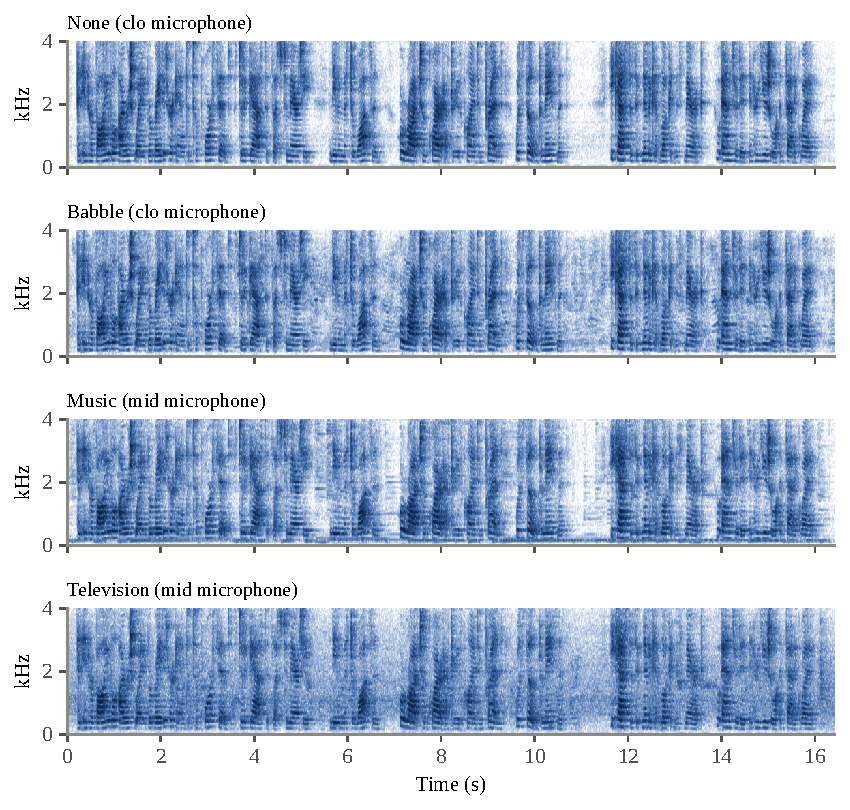
\includegraphics[width=0.66\textwidth]{fig3_voices_distractors.pdf}
\caption{Spectrograms of sentence \VExample{} in room \VRoom{} with the four background conditions, each from the closest microphone available for that condition.}\label{fig:dist}
\end{figure}

A practical problem appeared at once: the subset archives store absolute paths from the author's computer and also contain macOS metadata files (names starting with \texttt{.\_}), which are not audio. I extracted only the \texttt{.wav} files and skipped the metadata.

\textbf{Splits.} Each sentence appears up to 13 times, in different rooms, with different distractors and at different microphones. If the same sentence were in training and testing, a model could recognise the sentence and not the background. Every split in this report is therefore grouped by sentence.

\section{Events and background}
VOiCES labels backgrounds but not individual sound events, so for events I used ESC-10~\cite{esc}, the 10-class subset of ESC-50 with 40 five-second clips per class. I grouped the classes myself: dog, rooster, sneezing, crying baby and clock tick as \emph{events}, and rain, sea waves, crackling fire, helicopter and chainsaw as \emph{background}. Each clip is described by the mean and standard deviation of its MFCCs and deltas, and I used the five official folds.

\begin{table}[H]\centering\small\caption{ESC-10 results, official 5 folds, accuracy (\%) $\pm$ std.}\label{tab:esc}
\begin{tabular}{lccc}\toprule Classifier & Event vs background & 10 classes & 10-class macro F1\\\midrule
SVM (RBF) & 95.2 $\pm$ 3.1 & 77.8 $\pm$ 8.6 & 77.7 $\pm$ 8.4\\
Neural network (MLP) & 95.0 $\pm$ 3.2 & 75.5 $\pm$ 6.4 & 75.2 $\pm$ 6.0\\
Random forest & 93.8 $\pm$ 4.1 & 78.2 $\pm$ 3.5 & 77.5 $\pm$ 3.8\\
\bottomrule\end{tabular}\end{table}


Telling events from background is much easier than naming the class, which is expected, as my grouping mostly separates short sounds from continuous ones. The three models overlap once the fold spread is considered. Table~\ref{tab:conf} shows that the SVM mostly confuses noise-like sounds: clock tick with crackling fire, and helicopter with rain and sea waves.

\begin{table}[H]\centering\small\caption{ESC-10 confusion matrix of the SVM, pooled over the five folds (400 clips). Rows are true classes and columns are predictions.}\label{tab:conf}
\setlength{\tabcolsep}{3pt}\begin{tabular}{lcccccccccc}\toprule True & Saw & Clock & Fire & Baby & Dog & Heli & Rain & Rooster & Sea & Sneeze\\\midrule
Saw & 31 & 1 & 0 & 0 & 0 & 6 & 0 & 0 & 1 & 1\\
Clock & 0 & 23 & 7 & 2 & 4 & 1 & 1 & 0 & 1 & 1\\
Fire & 0 & 5 & 27 & 0 & 0 & 1 & 6 & 0 & 0 & 1\\
Baby & 0 & 0 & 0 & 36 & 3 & 0 & 0 & 0 & 0 & 1\\
Dog & 0 & 4 & 0 & 1 & 33 & 0 & 0 & 1 & 0 & 1\\
Heli & 0 & 1 & 1 & 0 & 0 & 25 & 6 & 0 & 5 & 2\\
Rain & 1 & 0 & 1 & 0 & 0 & 2 & 36 & 0 & 0 & 0\\
Rooster & 0 & 1 & 0 & 2 & 1 & 0 & 0 & 34 & 0 & 2\\
Sea & 0 & 0 & 0 & 0 & 1 & 2 & 4 & 0 & 32 & 1\\
Sneeze & 0 & 2 & 0 & 1 & 1 & 0 & 0 & 2 & 0 & 34\\
\bottomrule\end{tabular}\end{table}


\section{Background classification on VOiCES}
Here each file gets one of four labels: none, babble, music or television. I first used the same MFCC statistics (52 values). Since Figure~\ref{fig:dist} suggests that the background shows itself in the quiet frames, I added a second set of nine numbers that describe how the band energy (300--3400~Hz) is spread over the file: low percentiles relative to the loudest frames, the 10--90\% range, and how fast the energy changes. These need no VAD. The six classifiers from Mini Task 8 were used, with a small grid search inside each training fold.

\begin{table}[H]\centering\small\caption{Background classification on VOiCES (4 classes, 908 files). Accuracy and macro F1 (\%) over 5 folds grouped by sentence, mean $\pm$ std. Chance is 25\%.}\label{tab:bg}
\setlength{\tabcolsep}{4pt}\begin{tabular}{lcccc}\toprule & \multicolumn{2}{c}{MFCC statistics} & \multicolumn{2}{c}{+ energy levels}\\\cmidrule(lr){2-3}\cmidrule(lr){4-5}
Classifier & Accuracy & Macro F1 & Accuracy & Macro F1\\\midrule
SVM (RBF) & 72.6 $\pm$ 3.8 & 72.0 & 73.9 $\pm$ 2.1 & 73.3\\
Neural network (MLP) & 68.5 $\pm$ 3.9 & 68.1 & 72.0 $\pm$ 4.1 & 71.7\\
Logistic regression & 67.0 $\pm$ 3.3 & 66.3 & 72.6 $\pm$ 2.9 & 72.0\\
Random forest & 67.0 $\pm$ 2.0 & 65.8 & 68.5 $\pm$ 3.3 & 66.6\\
k-NN & 60.2 $\pm$ 4.1 & 57.7 & 60.3 $\pm$ 3.2 & 57.7\\
Gaussian naive Bayes & 63.0 $\pm$ 3.8 & 61.6 & 62.0 $\pm$ 3.1 & 60.1\\
\bottomrule\end{tabular}\end{table}


The SVM is best with both feature sets, at about 74\% against a chance level of 25\%. The energy-level features help logistic regression most (from 67.0\% to 72.6\%) and the MLP from 68.5\% to 72.0\%. For the SVM the gain is within the fold spread. k-NN and naive Bayes are clearly weaker. Every model does better in room rm2 than in rm1 (by 2.5 points for the SVM and 12 points for k-NN), while the microphone position changes the SVM's accuracy only between 70\% and 78\%.

\begin{table}[H]\centering\small\caption{Confusion matrix of the SVM with both feature sets, summed over the five folds. Rows are the true background.}\label{tab:bgconf}
\begin{tabular}{lcccc}\toprule True & None & Babble & Music & Television\\\midrule
None & 178 & 3 & 13 & 33\\
Babble & 0 & 200 & 7 & 21\\
Music & 21 & 9 & 177 & 24\\
Television & 37 & 33 & 36 & 116\\
\bottomrule\end{tabular}\end{table}


Television is the hard class: only 116 of 222 television files are right, and they are confused with all three other classes. It is also the class that the no-distractor files are most often mistaken for. My guess is that television contains both speech and music, and that it is often quiet, so it can look like any of the other three. Babble is the easiest (200 of 228).

\section{Reference labels for VAD}
VOiCES gives transcripts but, as far as I could find, no frame-level speech labels, and the subset does not include the clean source files. I therefore built a reference from the data itself:
\begin{enumerate}[nosep,leftmargin=*]
\item For each sentence and room, I took the no-distractor recording from the closest microphone.
\item I labelled it with an energy rule on the 300--3400~Hz band, with gaps under 90~ms closed and bursts under 50~ms removed.
\item I shifted these labels onto every other recording of the same sentence in that room, by cross-correlating the band envelopes.
\end{enumerate}
\VGroups{} sentence--room groups have a no-distractor recording, which gives \VLab{} labelled files. The alignment seems reliable: the normalised correlation peak is above \VPeak{} for 95\% of the files, and when one playback was recorded by several microphones, the estimated delays agree to within one 10~ms frame (checked on 44 such sessions).

This reference has two weaknesses. Short gaps between words are closed, so the labels are closer to phrase level, and about \VShare\% of the frames are speech. A detector that always says ``speech'' would already reach high accuracy and F1, so the false alarm rate is the more telling number here. Also, the labels come from an energy rule. To avoid favouring the energy-based method, the recording that produced a group's labels was never used as a test file.

\section{Speech and non-speech windows}
I cut each labelled file into 0.5~s windows with 50\% overlap and kept the windows that are at least 95\% speech or at most 5\% speech, which removes the ambiguous edges. Each window was described by MFCC statistics. Training and testing used four folds grouped by sentence.

\begin{table}[H]\centering\small\caption{Speech/non-speech classification of 0.5~s windows (22631 test windows, 92.4\% speech). Speech is the positive class.}\label{tab:win}
\begin{tabular}{lccccc}\toprule Classifier & Precision & Recall & F1 & Non-speech recall & Balanced acc.\\\midrule
SVM (RBF) & 99.0 & 99.2 & 99.1 & 87.2 & 93.2\\
Neural network (MLP) & 99.0 & 99.2 & 99.1 & 87.9 & 93.6\\
Logistic regression & 99.6 & 96.4 & 98.0 & 95.6 & 96.0\\
\bottomrule\end{tabular}\end{table}


All three models find almost all speech windows. The difference is in the pauses: the SVM and the MLP keep only 87--88\% of the non-speech windows, while logistic regression with balanced class weights keeps 95.6\% and has the best balanced accuracy. With no distractor every model is close to perfect (balanced accuracy above 99\%), so the errors come from the pauses that a distractor fills.

\section{Voice activity detection}
For the frame-level task I compared four methods: an adaptive energy threshold, a spectral entropy rule, and two frame classifiers (logistic regression and an MLP) on normalised MFCCs, deltas and a 310~ms local average. All four use a 200~ms median filter. The rule thresholds were tuned on the training folds, like the classifiers, and the energy threshold ended between 0.15 and 0.20 of the range. For the entropy rule the best value was the edge of my search range (0.9), so its result may be slightly better with a wider search.

\begin{table}[H]\centering\small\caption{Frame-level VAD on VOiCES, all test files pooled (4 folds grouped by sentence). Rates in \%.}\label{tab:vadv}
\begin{tabular}{lcccc}\toprule Method & F1 & Precision & Miss rate & False alarm rate\\\midrule
Energy threshold & 95.6 & 95.3 & 4.1 & 18.7\\
Spectral entropy & 88.3 & 85.7 & 9.0 & 59.9\\
Logistic regression (frames) & 96.7 & 95.5 & 2.1 & 18.4\\
Neural network (frames) & 97.0 & 95.9 & 1.9 & 16.6\\
\bottomrule\end{tabular}\end{table}


\begin{figure}[H]\centering
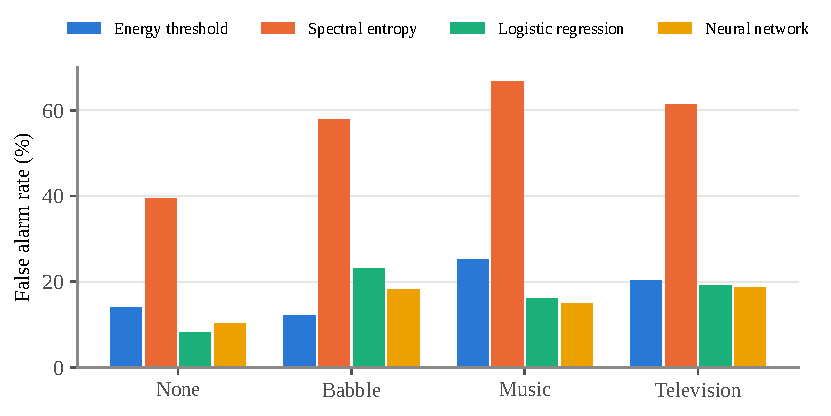
\includegraphics[width=0.72\textwidth]{fig5_voices_false_alarms.pdf}
\caption{False alarm rate of each method by background condition.}\label{fig:fa}
\end{figure}

The MLP is the best overall, with the fewest misses and false alarms. Logistic regression and the energy rule are close behind, and the spectral entropy rule is clearly worse, marking more than half of the pause frames as speech. Figure~\ref{fig:fa} shows that the ranking depends on the background. With music, the energy rule raises false alarms on a quarter of the pause frames, against 15\% for the MLP. With babble, the energy rule has the fewest false alarms (12\%) and logistic regression the most (23\%). The microphone position matters little: the MLP's false alarm rate stays between 16\% and 18\% at all four positions.

\begin{figure}[H]\centering
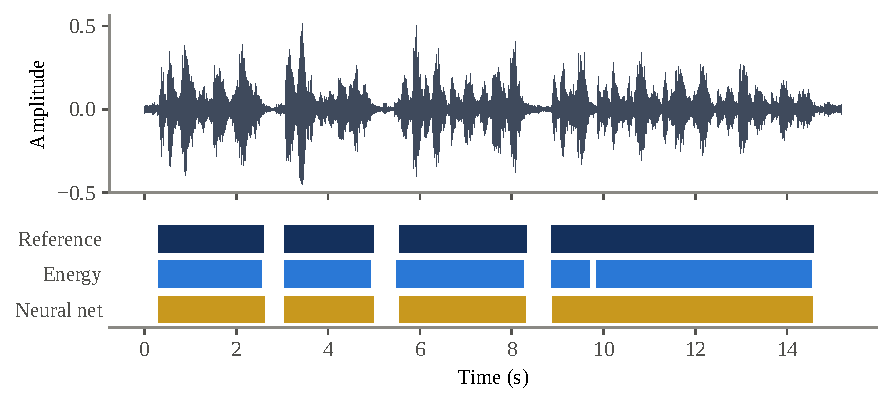
\includegraphics[width=0.88\textwidth]{fig4_voices_vad_example.pdf}
\caption{A test file with music at the far microphone. The MLP shown here was trained on all other sentences.}\label{fig:ex}
\end{figure}

\section{Discussion}
The two tasks behave differently. Background classification is hard: even the best model gets about a quarter of the files wrong, and television is mistaken for every other class. VAD looks easy at first because most frames are speech, but the false alarm rates of 17--19\% for the three better methods show that about a fifth of the pauses are still called speech. In both tasks the useful information is in the pauses, which is also where the methods differ.

The learned frame classifier was the most consistent across backgrounds. The energy rule was a surprisingly strong baseline in this subset, but it depends on how loud the distractor is, and it is weakest with music. I would choose the MLP, while keeping in mind that its lead over logistic regression and the energy rule is less than two points of F1.

\textbf{Limitations.}
\begin{itemize}[nosep,leftmargin=*]
\item The reference labels are my own construction. They are phrase-level and come from an energy rule, so they may agree more with energy-like decisions, even though the reference recordings were not used for testing.
\item I worked at 8~kHz, which drops the upper band. Television and music may be easier to separate at 16~kHz. I did not test this.
\item Only two rooms and the 90-degree position are in the subset, so the results do not cover other rooms or speaker angles.
\item ESC-10 events are a separate data set, so the events and the VOiCES backgrounds are not tested together.
\end{itemize}

A next step would be to repeat the frame classifier with pre-trained wav2vec 2.0 features~\cite{wav2vec} at 16~kHz, and to add the Python VAD from the class tutorial as a further baseline.

\section{Conclusion}
On the VOiCES subset, the SVM classified the four backgrounds with about 74\% accuracy, and television was the hardest class. Speech and non-speech windows were separated with up to 96\% balanced accuracy. For frame-level VAD, a small MLP on MFCC features gave an F1 of 97\% and the lowest false alarm rate, ahead of logistic regression and an energy rule, with spectral entropy clearly last. The main thing I learned is that with distant microphones the difficulty lies in the pauses, and that a VAD has to be judged by its false alarms and not only by accuracy.

\begingroup\small
\begin{thebibliography}{9}\setlength{\itemsep}{0pt}
\bibitem{voices} C. Richey et al., ``Voices Obscured in Complex Environmental Settings (VOICES) corpus,'' arXiv:1804.05053, 2018.
\bibitem{subset} Lab41, ``VOiCES-subset.'' \url{https://github.com/Lab41/VOiCES-subset}
\bibitem{readme} ``Dataset description,'' VOiCES README, IQT Labs. \url{https://iqtlabs.github.io/voices/Lab41-SRI-VOiCES_README}
\bibitem{esc} K. J. Piczak, ``ESC: Dataset for environmental sound classification,'' in \emph{Proc. ACM Multimedia}, 2015. \url{https://github.com/karolpiczak/ESC-50}
\bibitem{wav2vec} A. Baevski, H. Zhou, A. Mohamed and M. Auli, ``wav2vec 2.0: A framework for self-supervised learning of speech representations,'' arXiv:2006.11477, 2020.
\end{thebibliography}
\endgroup
\end{document}
